\documentclass[british]{article}
\usepackage[T1]{fontenc}
\usepackage[latin9]{inputenc}
\usepackage{geometry}
\geometry{verbose,tmargin=3.5cm,bmargin=3.5cm,lmargin=3cm,rmargin=3cm}
\usepackage{array}
%\usepackage{multirow}
\usepackage{amstext}
\usepackage{graphicx}
\usepackage{color}
\usepackage{caption}
%\usepackage{subfigure}

\newcommand{\tabincell}[2]{\begin{tabular}{@{}#1@{}}#2\end{tabular}}

\newcommand{\mytablefontsize}{9pt}
\newcommand{\mytablebaselineskip}{0.7}
\newcommand{\mytabcolsep}{5pt}

\newcommand{\medianInterval}[1]{}


\makeatletter

%%%%%%%%%%%%%%%%%%%%%%%%%%%%%% LyX specific LaTeX commands.
%% Because html converters don't know tabularnewline
\providecommand{\tabularnewline}{\\}

%%%%%%%%%%%%%%%%%%%%%%%%%%%%%% User specified LaTeX commands.

\title{The System Report for \emph{Sparkle} }
\author{ Automatically generated by \emph{Sparkle} (version: Sparkle\textunderscore SAT\textunderscore Challenge\textunderscore 2018) }

\makeatother

\usepackage{babel}
\begin{document}
\maketitle %


\section{Introduction}
\label{sec:Introduction}

\emph{Sparkle} \cite{Hoos15} is a multi-agent problem-solving platform based on Programming by Optimisation (PbO) \cite{Hoos12}, and would provide a number of effective algorithm optimisation techniques (such as automated algorithm configuration, portfolio-based algorithm selection, etc) to accelerate the existing solvers.

This experimental report is automatically generated by \emph{Sparkle}. This report presents the system status for \emph{Sparkle}.


\section{Experimental Preliminaries}
\label{sec:Experimental_Preliminaries}

In this section, we present the experimental preliminaries, including the list of solvers, the list of feature extractors, the list of instance classes, the information about experimental setup and the information about how to construct a portfolio-based algorithm selector in \emph{Sparkle}.

\subsection{Solvers}
\label{sec:Solvers}
There are 19 solver(s) submitted in \emph{Sparkle}, and the list of solver(s) is given as follows.


\begin{enumerate} 
\item \textbf{CaDiCaL}
\item \textbf{Lingeling}
\item \textbf{YalSAT}
\item \textbf{Dimetheus}
\item \textbf{gluHack}
\item \textbf{Minisat-v2.2.0-68-g37dc6c6}
\item \textbf{Riss7}
\item \textbf{Riss7-no-preprocessor}
\item \textbf{minisat-2.2.0\textunderscore PADC}
\item \textbf{BreakIDGlucoseSEL}
\item \textbf{UPLS}
\item \textbf{glucose-3.0\textunderscore PADC}
\item \textbf{CryptoMiniSatv5.5}
\item \textbf{glu\textunderscore mix}
\item \textbf{smallsat}
\item \textbf{ReasonLS}
\item \textbf{probSAT}
\item \textbf{SparrowToRiss-2018}
\item \textbf{CPSparrow}

\end{enumerate}


\subsection{Feature Extractors}
\label{sec:Feature_Extractors}
There are 1 feature extractor(s) submitted in \emph{Sparkle}, and the list of feature extractor(s) is given as follow.

\begin{enumerate}
\item \textbf{SAT-features-competition2012\textunderscore revised\textunderscore sparkle}

\end{enumerate}

\subsection{Instance Classes}
\label{sec:Instance_Classes}
There are 1356 instance(s) submitted in \emph{Sparkle}. All instance(s) are classified into 18 instance class(es), and the list of instance class(es) is given as follows.

\begin{enumerate}
\item \textbf{Balyo}, number of instances: 32
\item \textbf{Ehlers}, number of instances: 20
\item \textbf{Manthey}, number of instances: 33
\item \textbf{SC-past}, number of instances: 63
\item \textbf{Giraldez}, number of instances: 27
\item \textbf{Kojevnikov}, number of instances: 16
\item \textbf{SC2017-Main\textunderscore UNSAT}, number of instances: 127
\item \textbf{SC2017-Main\textunderscore SAT}, number of instances: 127
\item \textbf{SC2014-Crafted\textunderscore UNSAT}, number of instances: 128
\item \textbf{SR2015-Main\textunderscore UNSAT}, number of instances: 117
\item \textbf{SC2014-Crafted\textunderscore SAT}, number of instances: 124
\item \textbf{Elffers}, number of instances: 62
\item \textbf{Heule}, number of instances: 30
\item \textbf{SR2015-Main\textunderscore SAT}, number of instances: 169
\item \textbf{SC2014-APP\textunderscore SAT}, number of instances: 126
\item \textbf{SC2014-APP\textunderscore UNSAT}, number of instances: 149
\item \textbf{Balabanov}, number of instances: 3
\item \textbf{Wedler}, number of instances: 3

\end{enumerate}

\subsection{Experimental Setup}
\label{sec:Experimental_Setup}

\textbf{Feature computation:} We use all the feature extractors which are presented above to compute the feature vector for each instance. Each feature extractor will compute a feature vector for each instance. The final feature vector is the combination of all computed feature vectors. The cutoff time for feature vector computation on each instance is set to 90 seconds. The memory limit for feature vector computation on each instance is set to 32768 MB.

\textbf{Performance computation:} Each solver will run one time on each instance. The cutoff time for each performance computation run is set to 5000 seconds. The memory limit for each performance computation run is set to 8192 MB.

\subsection{Constructing Portfolio-Based Algorithm Selector}
\label{sec:Portfolio}

\emph{Sparkle} runs all the feature extractors to compute the feature vector for each instance, and store the resulting feature data (feature vectors for all instances) in the system. Also, \emph{Sparkle} runs all the solvers to solve each instance, and store the resulting performance data in the system. After the feature-related and the performance-related experiments are finished, by utilising the feature data and the performance data, \emph{Sparkle} uses \emph{AutoFolio} \cite{LinEtAl15} to automatically construct a portfolio-based algorithm selector in the system.

\subsection{Marginal Contribution}
\label{sec:Marginal_Contribution}

Since the primary goal of \emph{Sparkle} is to analyse the contribution of each solver to the real state of the art, \emph{Sparkle} utilises the concept of marginal contribution \cite{XuEtAl12} to measure each solver's contribution to the \textbf{perfect portfolio selector}, also known as Virtual Best Solver (\emph{VBS}), and the \textbf{actual portfolio selector}.

Now we give the protocol for calculating each solver's marginal contribution. Assume that we have a set of solvers $S$ and a portfolio selector $P$ constructed based on a subset of $S$. In this report, the performance of a solver or portfolio selector is measured via the the penalised average runtime (PAR2), which conforms with the measurement used in SAT Competitions. Let $\mathit{par2(P)}$ denote the PAR2 value achieved by leveraging the complementary strengths of the algorithms in $P$.

The absolute marginal contribution (Abs\textunderscore Margi\textunderscore Contr) for solver $s$ is calculated as 
\begin{equation}
amc(s)=\left\{
\begin{array}{ccl}
log_{10}{\frac{\mathit{par2(P\textbackslash \{s\})}}{\mathit{par2(P)}}} & & \mathit{par2(P\textbackslash \{s\})}> \mathit{par2(P)} \\
& & \\
0 & & \text{else}
\end{array} \right.
\end{equation}


Then, for each solver $s$, we calculate the relative marginal contribution (Rel\textunderscore Margi\textunderscore Contr), which is propositional to the absolute marginal contribution, with normalisation. The relative marginal contribution for solver $s$ is calculated as 
\begin{equation}
\mathit{rmc(s)}=\frac{\mathit{amc(s)}}{\sum_{s' \in S}{amc(s')}}
\end{equation}

Finally, the contribution of each solver is evaluated by the relative marginal contribution.

\section{Experimental Results}
\label{sec:Experimental_Results}

In this section, the related experimental results in \emph{Sparkle} are presented and analysed.

\subsection{PAR2 Ranking List}
\label{sec:PAR2_Ranking}

The ranking list with regards to the PAR2 value for solvers is given in Table \ref{tab:PenaltyTimeRankingList}. Also, the PAR2 values for the \textbf{perfect portfolio selector} and the \textbf{actual portfolio selector} are given in Table \ref{tab:PenaltyTimeForPerfectAndActual}.

\begin{table} [t]
\center
\caption{The ranking list with regards to the PAR2 value for solvers.}\label{tab:PenaltyTimeRankingList}
\fontsize{\mytablefontsize}{\mytablebaselineskip\baselineskip}\selectfont\setlength{\tabcolsep}{\mytabcolsep}
{
\begin{tabular}{rlr}
\hline
$\#$Rank & Solver & PAR2 \\
\hline
1 & CryptoMiniSatv5.5 & 2463.982073\\
2 & ReasonLS & 2620.041987\\
3 & smallsat & 2910.422549\\
4 & glu\textunderscore mix & 2976.411382\\
5 & Lingeling & 3312.241490\\
6 & BreakIDGlucoseSEL & 3349.265918\\
7 & CaDiCaL & 3361.921577\\
8 & SparrowToRiss-2018 & 3492.195292\\
9 & Riss7 & 3578.461102\\
10 & Riss7-no-preprocessor & 3589.350130\\
11 & glucose-3.0\textunderscore PADC & 3863.798855\\
12 & Minisat-v2.2.0-68-g37dc6c6 & 4563.354665\\
13 & gluHack & 4584.416739\\
14 & minisat-2.2.0\textunderscore PADC & 4588.428186\\
15 & UPLS & 7715.254125\\
16 & CPSparrow & 8034.144492\\
17 & YalSAT & 8344.633261\\
18 & Dimetheus & 9477.172203\\
19 & probSAT & 9499.151058\\

\hline
\end{tabular}
}
\end{table}

\begin{table} [t]
\center
\caption{The PAR2 values for the perfect portfolio selector, and the actual portfolio selector in \emph{Sparkle}.}\label{tab:PenaltyTimeForPerfectAndActual}
\fontsize{\mytablefontsize}{\mytablebaselineskip\baselineskip}\selectfont\setlength{\tabcolsep}{\mytabcolsep}
{
\begin{tabular}{lr}
\hline
Solver & PAR2 \\
\hline
Perfect Portfolio Selector & 413.835616 \\
Actual Portfolio Selector & 1285.765832 \\
\hline
\end{tabular}
}
\end{table}

For each solver, we present the PAR2 value for the perfect portfolio selector excluding the corresponding solver, which can be seen in Table \ref{tab:perfectPortfolioPenaltyTimeList}. Also, for each solver, we present the PAR2 value for the actual portfolio selector excluding the corresponding solver, which can be seen in Table \ref{tab:actualPortfolioPenaltyTimeList}.

\begin{table} [t]
\center
\caption{The list of PAR2 values for the perfect portfolio selectors excluding each solver in \emph{Sparkle}.}\label{tab:perfectPortfolioPenaltyTimeList}
\fontsize{\mytablefontsize}{\mytablebaselineskip\baselineskip}\selectfont\setlength{\tabcolsep}{\mytabcolsep}
{
\begin{tabular}{lr}
\hline
Solver & PAR2 \\
\hline
Perfect Portfolio Selector excluding \emph{Dimetheus} & 413.835616 \\ 
Perfect Portfolio Selector excluding \emph{probSAT} & 413.835616 \\ 
Perfect Portfolio Selector excluding \emph{YalSAT} & 413.897473 \\ 
Perfect Portfolio Selector excluding \emph{CPSparrow} & 414.176955 \\ 
Perfect Portfolio Selector excluding \emph{Riss7-no-preprocessor} & 414.249978 \\ 
Perfect Portfolio Selector excluding \emph{SparrowToRiss-2018} & 414.639741 \\ 
Perfect Portfolio Selector excluding \emph{minisat-2.2.0\textunderscore PADC} & 415.935313 \\ 
Perfect Portfolio Selector excluding \emph{Riss7} & 416.562981 \\ 
Perfect Portfolio Selector excluding \emph{gluHack} & 417.872851 \\ 
Perfect Portfolio Selector excluding \emph{Minisat-v2.2.0-68-g37dc6c6} & 422.462030 \\ 
Perfect Portfolio Selector excluding \emph{UPLS} & 426.610130 \\ 
Perfect Portfolio Selector excluding \emph{glu\textunderscore mix} & 429.338661 \\ 
Perfect Portfolio Selector excluding \emph{CaDiCaL} & 435.294816 \\ 
Perfect Portfolio Selector excluding \emph{glucose-3.0\textunderscore PADC} & 436.069935 \\ 
Perfect Portfolio Selector excluding \emph{ReasonLS} & 442.137667 \\ 
Perfect Portfolio Selector excluding \emph{Lingeling} & 446.187559 \\ 
Perfect Portfolio Selector excluding \emph{BreakIDGlucoseSEL} & 447.863607 \\ 
Perfect Portfolio Selector excluding \emph{smallsat} & 451.887473 \\ 
Perfect Portfolio Selector excluding \emph{CryptoMiniSatv5.5} & 453.701620 \\ 

\hline
\end{tabular}
}
\end{table}

\begin{table} [t]
\center
\caption{The list of PAR2 values for the actual portfolio selectors excluding each solver in \emph{Sparkle}.}\label{tab:actualPortfolioPenaltyTimeList}
\fontsize{\mytablefontsize}{\mytablebaselineskip\baselineskip}\selectfont\setlength{\tabcolsep}{\mytabcolsep}
{
\begin{tabular}{lr}
\hline
Solver & PAR2 \\
\hline
Actual Portfolio Selector excluding \emph{Riss7} & 1285.765832 \\ 
Actual Portfolio Selector excluding \emph{BreakIDGlucoseSEL} & 1324.842419 \\ 
Actual Portfolio Selector excluding \emph{YalSAT} & 1383.187819 \\ 
Actual Portfolio Selector excluding \emph{Dimetheus} & 1387.401922 \\ 
Actual Portfolio Selector excluding \emph{glucose-3.0\textunderscore PADC} & 1395.762678 \\ 
Actual Portfolio Selector excluding \emph{minisat-2.2.0\textunderscore PADC} & 1400.234514 \\ 
Actual Portfolio Selector excluding \emph{ReasonLS} & 1407.736609 \\ 
Actual Portfolio Selector excluding \emph{Riss7-no-preprocessor} & 1409.388121 \\ 
Actual Portfolio Selector excluding \emph{Minisat-v2.2.0-68-g37dc6c6} & 1410.017603 \\ 
Actual Portfolio Selector excluding \emph{CaDiCaL} & 1439.474168 \\ 
Actual Portfolio Selector excluding \emph{gluHack} & 1440.323629 \\ 
Actual Portfolio Selector excluding \emph{UPLS} & 1451.370756 \\ 
Actual Portfolio Selector excluding \emph{SparrowToRiss-2018} & 1461.093153 \\ 
Actual Portfolio Selector excluding \emph{CPSparrow} & 1467.619309 \\ 
Actual Portfolio Selector excluding \emph{Lingeling} & 1520.733261 \\ 
Actual Portfolio Selector excluding \emph{probSAT} & 1537.504989 \\ 
Actual Portfolio Selector excluding \emph{glu\textunderscore mix} & 1577.560518 \\ 
Actual Portfolio Selector excluding \emph{CryptoMiniSatv5.5} & 1645.305097 \\ 
Actual Portfolio Selector excluding \emph{smallsat} & 1679.208877 \\ 

\hline
\end{tabular}
}
\end{table}


\subsection{Relative Marginal Contribution Ranking List}
\label{sec:Relative_Marginal_Contribution_Ranking}

\emph{Sparkle} uses the concept of marginal contribution \cite{XuEtAl12} to measure each solver's contribution to the \textbf{perfect portfolio selector} and to the \textbf{actual portfolio selector}. In this report, we use the relative marginal contribution to evaluate each solver's contribution.

The solver ranking list via relative marginal contribution for solvers with regards to the \textbf{perfect portfolio selector} is given in Table \ref{tab:solverPerfectRankingList}. Also, the solver ranking list via relative marginal contribution for solvers with regards to the \textbf{actual portfolio selector} is given in Table \ref{tab:solverActualRankingList}.

\begin{table} [t]
\center
\caption{Solver ranking list via relative marginal contribution for solvers with regards to the \textbf{perfect portfolio selector}.}\label{tab:solverPerfectRankingList}
\fontsize{\mytablefontsize}{\mytablebaselineskip\baselineskip}\selectfont\setlength{\tabcolsep}{\mytabcolsep}
{
\begin{tabular}{rlrr}
\hline
$\#$Rank & Solver & Rel\textunderscore Margi\textunderscore Contr & Abs\textunderscore Margi\textunderscore Contr \\
\hline
1 & CryptoMiniSatv5.5 & 0.149223 & 0.039942 \\ 
2 & smallsat & 0.142723 & 0.038202 \\ 
3 & BreakIDGlucoseSEL & 0.128210 & 0.034318 \\ 
4 & Lingeling & 0.122127 & 0.032690 \\ 
5 & ReasonLS & 0.107333 & 0.028730 \\ 
6 & glucose-3.0\textunderscore PADC & 0.084912 & 0.022728 \\ 
7 & CaDiCaL & 0.082025 & 0.021956 \\ 
8 & glu\textunderscore mix & 0.059671 & 0.015972 \\ 
9 & UPLS & 0.049327 & 0.013203 \\ 
10 & Minisat-v2.2.0-68-g37dc6c6 & 0.033474 & 0.008960 \\ 
11 & gluHack & 0.015752 & 0.004216 \\ 
12 & Riss7 & 0.010658 & 0.002853 \\ 
13 & minisat-2.2.0\textunderscore PADC & 0.008211 & 0.002198 \\ 
14 & SparrowToRiss-2018 & 0.003150 & 0.000843 \\ 
15 & Riss7-no-preprocessor & 0.001624 & 0.000435 \\ 
16 & CPSparrow & 0.001338 & 0.000358 \\ 
17 & YalSAT & 0.000243 & 0.000065 \\ 
18 & Dimetheus & 0.000000 & 0.000000 \\ 
19 & probSAT & 0.000000 & 0.000000 \\ 

\hline
\end{tabular}
}
\end{table}

\begin{table} [t]
\center
\caption{Solver ranking list via relative marginal contribution for solvers with regards to the \textbf{actual portfolio selector}.}\label{tab:solverActualRankingList}
\fontsize{\mytablefontsize}{\mytablebaselineskip\baselineskip}\selectfont\setlength{\tabcolsep}{\mytabcolsep}
{
\begin{tabular}{rlrr}
\hline
$\#$Rank & Solver & Rel\textunderscore Margi\textunderscore Contr & Abs\textunderscore Margi\textunderscore Contr \\
\hline
1 & smallsat & 0.116401 & 0.115943 \\ 
2 & CryptoMiniSatv5.5 & 0.107508 & 0.107085 \\ 
3 & glu\textunderscore mix & 0.089175 & 0.088824 \\ 
4 & probSAT & 0.077962 & 0.077655 \\ 
5 & Lingeling & 0.073179 & 0.072891 \\ 
6 & CPSparrow & 0.057679 & 0.057452 \\ 
7 & SparrowToRiss-2018 & 0.055735 & 0.055516 \\ 
8 & UPLS & 0.052824 & 0.052616 \\ 
9 & gluHack & 0.049493 & 0.049298 \\ 
10 & CaDiCaL & 0.049236 & 0.049042 \\ 
11 & Minisat-v2.2.0-68-g37dc6c6 & 0.040221 & 0.040063 \\ 
12 & Riss7-no-preprocessor & 0.040026 & 0.039869 \\ 
13 & ReasonLS & 0.039515 & 0.039360 \\ 
14 & minisat-2.2.0\textunderscore PADC & 0.037185 & 0.037039 \\ 
15 & glucose-3.0\textunderscore PADC & 0.035791 & 0.035650 \\ 
16 & Dimetheus & 0.033171 & 0.033040 \\ 
17 & YalSAT & 0.031845 & 0.031719 \\ 
18 & BreakIDGlucoseSEL & 0.013054 & 0.013002 \\ 
19 & Riss7 & 0.000000 & 0.000000 \\ 

\hline
\end{tabular}
}
\end{table}


Solver ranking list via relative marginal contribution for solvers with regards to the \textbf{actual portfolio selector} is given as follows.




\subsection{Scatter Plot Analysis}

The empirical comparison between the actual portfolio selector in \emph{Sparkle} and single best solver (\emph{SBS}) is presented in Figure \ref{fig:sparkle_vs_sbs}. Also, the empirical comparison between the actual portfolio selector in \emph{Sparkle} and \emph{VBS} (i.e., the perfect portfolio selector) is presented in Figure \ref{fig:sparkle_vs_vbs}.

%\begin{figure}[t]
%\begin{minipage}{0.5\linewidth}
%\noindent \begin{centering}
%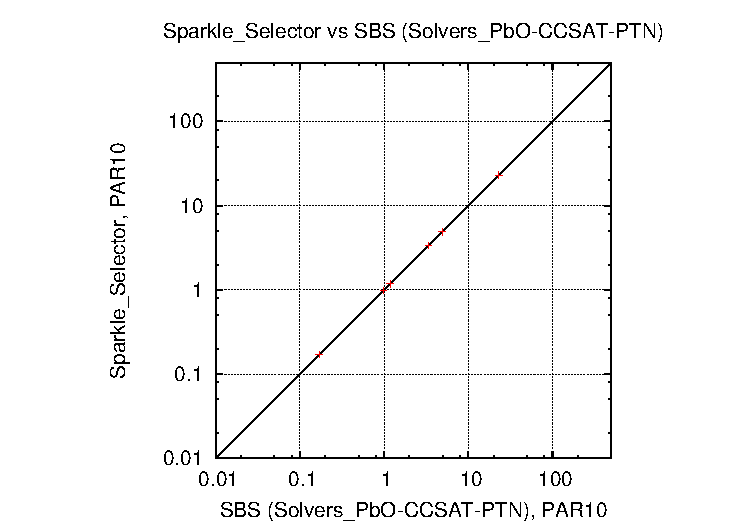
\includegraphics[width=0.6\textwidth]{figure_portfolio_selector_sparkle_vs_sbs}
%\par\end{centering}
%\caption{Empirical comparison between the actual portfolio selector in \emph{Sparkle} and \emph{SBS}.}\label{fig:sparkle_vs_sbs}
%\end{minipage}

%\begin{minipage}{0.5\linewidth}
%\noindent \begin{centering}
%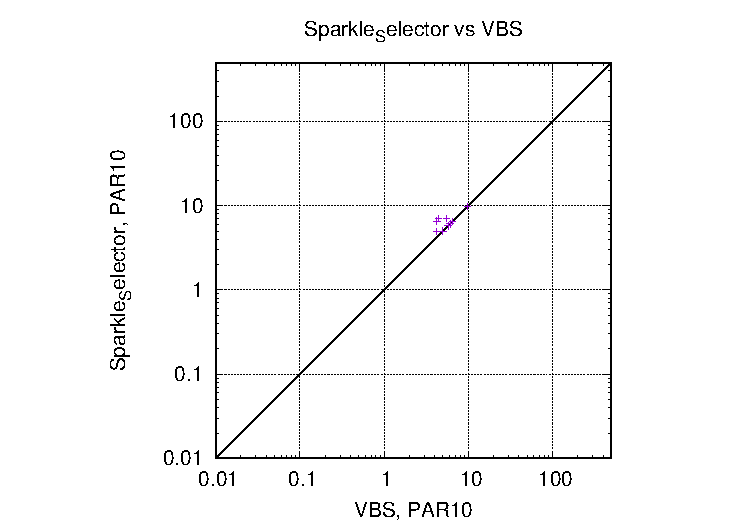
\includegraphics[width=0.6\textwidth]{figure_portfolio_selector_sparkle_vs_vbs}
%\par\end{centering}
%
%\end{minipage}
%\end{figure}

\begin{figure}[t]
\noindent \begin{centering}
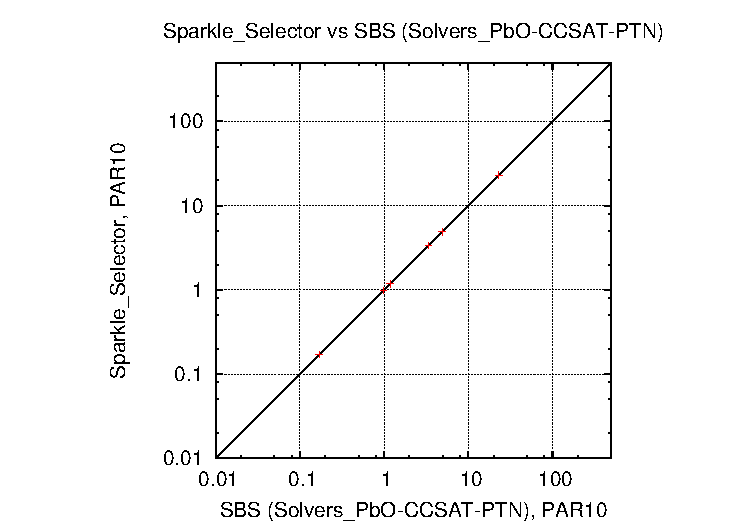
\includegraphics[width=0.6\textwidth]{figure_portfolio_selector_sparkle_vs_sbs}
% \includegraphics[width=0.8\textwidth]{fittedModels}
\par\end{centering}

\caption{Empirical comparison between the actual portfolio selector in \emph{Sparkle} and \emph{SBS}.}\label{fig:sparkle_vs_sbs}
\end{figure}

\begin{figure}[t]
\noindent \begin{centering}
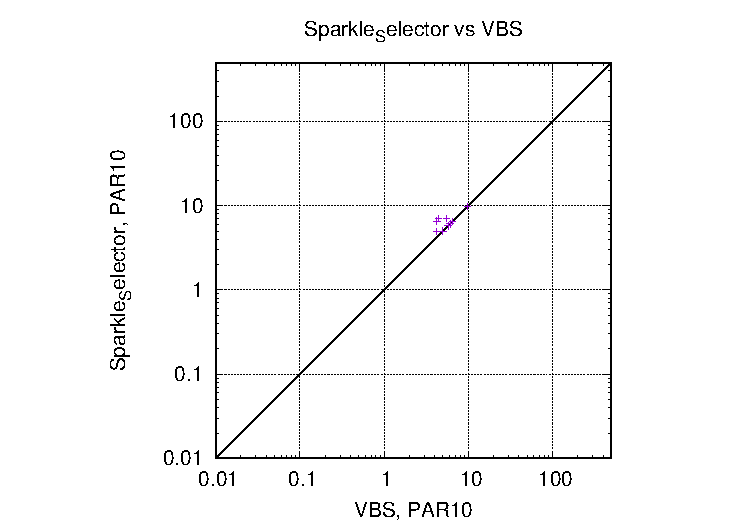
\includegraphics[width=0.6\textwidth]{figure_portfolio_selector_sparkle_vs_vbs}
% \includegraphics[width=0.8\textwidth]{fittedModels}
\par\end{centering}

\caption{Empirical comparison between the actual portfolio selector in \emph{Sparkle} and \emph{VBS}.}\label{fig:sparkle_vs_vbs}
\end{figure}



\bibliographystyle{plain}
\bibliography{Sparkle_Report}

\end{document}
